\chapter{Implementación}
\label{capitulo6}
\lhead{Capítulo 6. \emph{Dataset local}}


\section{Introducción}
El objetivo de este capítulo es explicar la elaboración de un dataset visual inercial, a través de la construcción de un robot prototipo.
\clearpage



\section{Descripción general}\label{seccion-corte}

La estimación de odometría por medio de la fusión visual inercial fue desarrollada utilizando C++ como lenguaje de programación y ROS para la aplicación de los filtros inerciales y la visualización del movimiento del robot. Este programa utiliza un sólo hilo de ejecución, de forma que la odometría se estima de forma secuencial, pasando primero por estimar la orientación del robot utilizando el filtro inercial, y luego a estimar la traslación a partir de los residuales inerciales y la cámara. El formato de entrada de las imágenes y de los datos de la IMU fueron tomados de acuerdo al formato empleado en el EUROC Mav dataset.

En cuanto al dataset local realizado, también fue implementado utilizando C++ como lenguaje de programación, y utilizando una raspberry pi 3 para la adquisición de los datos de la imu y de la cámara, y utilizando 4 hilos de ejecución.


\section{Componentes de hardware}

\begin{figure}[H]
	\centering
	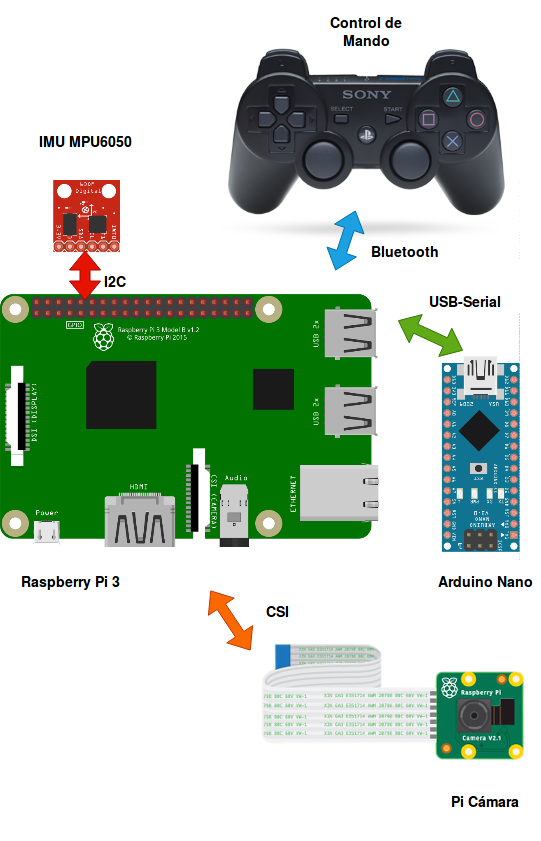
\includegraphics[width=0.7\textwidth]{HardwareRobot}
	\caption[Componentes de Hardware del robot]{Componentes de Hardware del robot.}
	\label{imagen:HardwareRobot}
\end{figure}

Con el empleo de la IMU es posible obtener los cambios de orientación de la cámara y de su aceleración, siempre y cuando se encuentren sincronizadas las mediciones. Bajo esta restricción se tiene el residual de orientación de la IMU (${R}_{RES/IMU}$) , el cual representa el cambio de orientación de la IMU entre el frame actual y el anterior, tal como se presenta en la ecuación \ref{eq:residualIMU}.

\begin{table}[htbp]
	\caption{Presupuesto del robot prototipo}
	\begin{tabular}{|l|c|c|c|}
		\hline
		\multicolumn{1}{|c|}{\textbf{Componente}} & \textbf{Cantidad} & \textbf{Valor (\$)} & \textbf{Precio Total (\$)} \\ \hline
		Arduino Nano 328p & 1 & 1.9 & 1.9 \\ \hline
		Batería Litio Sony G5 18650  2200mAh  & 12 & 2.0 & 24.0 \\ \hline
		Caja Acrílico Robot Diferencial & 1 & 25.0 & 25.0 \\ \hline
		Case Raspberry Pi 3 & 1 & 2.0 & 2.0 \\ \hline
		Caster & 1 & 4.0 & 4.0 \\ \hline
		Comparador LM311 & 2 & 0.1 & 0.2 \\ \hline
		Conectores y Cableado & 1 & 2.0 & 2.0 \\ \hline
		Driver STA6940M & 2 & 5.0 & 10.0 \\ \hline
		Ejes, Rolineras, Retenedores, Tornillos & 1 & 8.0 & 8.0 \\ \hline
		Fotoreceptor-Fotoemisor Impresora & 2 & 0.2 & 0.4 \\ \hline
		Frente Metálico & 1 & 1.0 & 1.0 \\ \hline
		Fusible 1A  Modelo  Americano & 2 & 0.1 & 0.2 \\ \hline
		Fusible 350 mA Modelo Europeo & 1 & 0.1 & 0.1 \\ \hline
		Impresión Engranajes y Rueda Encoder & 1 & 2.0 & 2.0 \\ \hline
		IMU MPU6050 & 1 & 0.6 & 0.6 \\ \hline
		Joystick PS3 & 1 & 10.0 & 10.0 \\ \hline
		Mini DC Buck Converter MP2307 & 2 & 0.4 & 0.8 \\ \hline
		Motor Mabuchi C2162-60006 19-24v Hp & 4 & 3.5 & 14.0 \\ \hline
		PCB Control Bajo Nivel & 1 & 10.0 & 10.0 \\ \hline
		Pi Camera  v1.2 & 1 & 7.2 & 7.2 \\ \hline
		Raspberry Pi 3 & 1 & 35.0 & 35.0 \\ \hline
		Rueda de Goma 7.48 mm de Diámetro & 2 & 4.0 & 8.0 \\ \hline
		& \multicolumn{1}{l|}{\textbf{Total (\$)}} & \multicolumn{1}{l|}{} & \textbf{166.44} \\ \hline
	\end{tabular}
	\label{PresupuestoRobot}
\end{table}







